\documentclass[UTF8]{article} 
\usepackage{geometry} 
%\usepackage{notestex}
\usepackage{amsmath,amsthm,amssymb,graphicx,mathtools,forest,float,color}
\graphicspath{{./figs/}}
\usepackage{wrapfig}

\usepackage{tikz}
\usepackage{circuitikz}
\usepackage{pgfplots} 
\pgfplotsset{width=10cm,compat=1.9} 
\usepgfplotslibrary{external} 
\tikzexternalize 
\usetikzlibrary{positioning}

\usepackage{hyperref}
\hypersetup{colorlinks,linkcolor=blue}
 
%\newcommand{\n}{\mathbb{N}}
%\newcommand{\z}{\mathbb{Z}}
%\newcommand{\q}{\mathbb{Q}}
%\newcommand{\cx}{\mathbb{C}}
%\newcommand{\real}{\mathbb{R}}
%%\newcommand{\field}{\mathbb{F}}
%\newcommand{\ita}[1]{\textit{#1}}
%\newcommand{\com}[2]{#1\backslash#2}
%\newcommand{\oneton}{\{1,2,3,...,n\}}
%\newcommand\idea[1]{\begin{gather*}#1\end{gather*}}
%\newcommand\ef{\ita{f} }
%\newcommand\eff{\ita{f}}
%\newcommand\proofs[1]{\begin{proof}#1\end{proof}}
%\newcommand\inv[1]{#1^{-1}}
%\newcommand\setb[1]{\{#1\}}
%\newcommand\en{\ita{n }}
%\newcommand{\vbrack}[1]{\langle #1\rangle}

\newtheorem{theo}{Theorem}
\newenvironment{theorem}[2][Theorem]{\begin{trivlist}
\item[\hskip \labelsep {\bfseries #1}\hskip \labelsep {\bfseries }]}{\end{trivlist}}
\newenvironment{lemma}[2][Lemma]{\begin{trivlist}
\item[\hskip \labelsep {\bfseries #1}\hskip \labelsep {\bfseries #2.}]}{\end{trivlist}}
\newenvironment{exercise}[2][Exercise]{\begin{trivlist}
\item[\hskip \labelsep {\bfseries #1}\hskip \labelsep {\bfseries #2.}]}{\end{trivlist}}
\newenvironment{reflection}[2][Reflection]{\begin{trivlist}
\item[\hskip \labelsep {\bfseries #1}\hskip \labelsep {\bfseries #2.}]}{\end{trivlist}}
\newenvironment{proposition}[2][Proposition]{\begin{trivlist}
\item[\hskip \labelsep {\bfseries #1}\hskip \labelsep {\bfseries #2.}]}{\end{trivlist}}
\newenvironment{corollary}[2][Corollary]{\begin{trivlist}
\item[\hskip \labelsep {\bfseries #1}\hskip \labelsep {\bfseries #2.}]}{\end{trivlist}}



\begin{document}


 
%\maketitle

\begin{titlepage}
\newcommand{\HRule}{\rule{\linewidth}{0.5mm}} % Defines a new command for the horizontal lines, change thickness here

\center % Center everything on the page

%----------------------------------------------------------------------------------------
%	HEADING SECTIONS
%----------------------------------------------------------------------------------------

\textsc{\LARGE City University of Hong Kong}\\[1.5cm] % Name of your university/college
\textsc{\Large AP Courses Review Notes}\\[0.5cm] 		% Major heading such as course name
\textsc{\large {AP2212/AP2213}}\\[0.5cm] 						% Minor heading such as course title

%----------------------------------------------------------------------------------------
%	TITLE SECTION
%----------------------------------------------------------------------------------------

\HRule \\[0.4cm]
{ \huge \bfseries  \textsf{(Advanced) Measurement and Instrumentation} }\\[0.4cm] % Title of your document
\rightline{2017--2018 Semester A/B}
\rightline{{\bfseries \textsf{Version 0.2}} }
\HRule \\[1.5cm]

%----------------------------------------------------------------------------------------
%	AUTHOR SECTION
%----------------------------------------------------------------------------------------

\begin{minipage}{0.4\textwidth}
\begin{flushleft} \large
\emph{Author:}\\
 Zezhu \textsc{Wei}
\end{flushleft}
\end{minipage}
~
\begin{minipage}{0.4\textwidth}
\begin{flushright} \large
\emph{Instructor:} \\
Sai Tak \textsc{CHU} % Supervisor's Name
\end{flushright}
\end{minipage}\\[2cm]

% If you don't want a supervisor, uncomment the two lines below and remove the section above
%\Large \emph{Author:}\\
%John \textsc{Smith}\\[3cm] % Your name

%----------------------------------------------------------------------------------------
%	DATE SECTION
%----------------------------------------------------------------------------------------


{\large \today}\\[2cm] % Date, change the \today to a set date if you want to be precise

%----------------------------------------------------------------------------------------
%	LOGO SECTION
%----------------------------------------------------------------------------------------
\vspace{5cm}
%
\includegraphics[scale=0.5]{figures/CityU_full_logo_2015.pdf}\\[1cm] % Include a department/university logo - this will require the graphicx package
%
\includegraphics[scale=0.5]{figures/CityU_logo_2015.eps}\\[1cm] % Include a department/university logo - this will require the graphicx package


%----------------------------------------------------------------------------------------

\vfill % Fill the rest of the page with whitespace
\end{titlepage}
\tableofcontents

\newpage
\section{Circuit Analysis}
\subsection{Basic elements in Circuit}
\subsubsection{Sources}
\begin{itemize}
\item Ideal Current Source
\begin{figure}[H]
  \begin{center}    
    \begin{circuitikz}[scale=0.8]
     	\draw (0,0) to [isource] (2,0);
        \draw (2,0) to [sI] (4,0);
    \end{circuitikz}
    \caption{Ideal Current Sources}
  \end{center}
\end{figure}

\begin{theorem}[Ideal Current Sources]
~ {For the ideal current source, the \textbf{internal resistance is regraded as infinity}, which means that a role of \textbf{open circuit} in analysis.}
\end{theorem}

\item Voltage Source
\begin{figure}[H]
  \begin{center}    
    \begin{circuitikz}[scale=0.8]
     	\draw (0,0) to [esource] (2,0);
        \draw (2,0) to [sV] (4,0);
    \end{circuitikz}
    \caption{Ideal Voltage Sources}
  \end{center}
\end{figure}

\begin{theorem}[Ideal Voltage Sources]
~ {For the ideal voltage source, the \textbf{internal resistance is regraded as zero}, which means that a role of \textbf{short circuit} in analysis.}
\end{theorem}

\begin{theorem}[Root-mean-square in Different Phase]
~ {When the voltage and the current are out of phase, say $V=V_P\sin \omega t$ and $i=i_P\sin (\omega t+\phi)$, then the rms power $P_{rms}=V_{rms}i_{rms} \cos \phi$}\\
 {Proof:}
\begin{align*}
P_{ave} &= \dfrac{V_P i_P}{\pi}\displaystyle\int_{0}^{\pi}\sin \omega t \sin (\omega t+\phi)d\omega t \\
&= \dfrac{V_P i_P}{2\pi}\displaystyle\int_{0}^{\pi}[\cos \phi - \cos (2\omega t+\phi )]d\omega t \\
&= \dfrac{V_P i_P}{2\pi}[\cos \phi - \frac{1}{2}\sin (2\omega t+\phi )]|_{0}^{\pi} \\
&= \dfrac{V_P i_P}{2} \cos \phi = \dfrac{V_P}{\sqrt{2}}\cdot \dfrac{i_P}{\sqrt{2}} \cos \phi \\
&= V_{rms}i_{rms} \cos \phi 
\end{align*}
\end{theorem}
\end{itemize}

\subsubsection{Impedance}
First, let's give the basic relation between impedance $Z$, resistance $R$ and reactance $X$:

%\begin{center}
%\begin{tikzpicture}[scale=1.25]%,cap=round,>=latex]
%\coordinate [label=left:$~$] (A) at (-1.5cm,-1.cm);
%\coordinate [label=right:$~$] (C) at (1.5cm,-1.0cm);
%\coordinate [label=above:$~$] (B) at (1.5cm,1.0cm);
%\draw (A) -- node[left] {$Impedance ~ Z$} (B) -- node[right] {$Reactance ~ X$} (C) -- node[below] %{$Resistance ~ R$} (A);
%\draw (1.25cm,-1.0cm) rectangle (1.5cm,-0.75cm);
%\end{tikzpicture}
%\end{center}

$$Z=R+jX=R+j \left( \omega L-\dfrac{1}{\omega C} \right)$$
%\begin{itemize}
\paragraph{Resistance}
%\begin{theorem}[Resistance]
%\item Resistance
\begin{figure}[H]
  \begin{center}    
    \begin{circuitikz}[scale=0.8]
     	\draw (0,0) to [R] (2,0);
        \draw (2,0) to [european resistor] (4,0);
    \end{circuitikz}
    \caption{Resistance}
  \end{center}
\end{figure}

%\begin{theorem}[Resistance]
~ {For the resistance, the value of resistance is the \textbf{real part} value of its impedance in circuit, which also suggests that \textbf{resistor dissipate energy}.}
$$\textit{Impedance}=R$$
 {Resistances are in \textbf{series or parallel} in circuit, the equivalent resistance given by:}
 \begin{align*}
\textit{Series: }&R_{12}=R_1+R_2 \\
\textit{Parallel: }&\dfrac{1}{R_{12}}=\dfrac{1}{R_1}+\dfrac{1}{R_2} \textit{ or } R_{12}=\dfrac{R_1R_2}{R_1+R_2}
\end{align*}
%\end{theorem}

%\paragraph{•}
%\item Capacitor
\paragraph{Capacitor}
\begin{figure}[H]
  \begin{center}    
    \begin{circuitikz}[scale=0.8]
     	\draw (0,0) to [C] (2,0);
    \end{circuitikz}
    \caption{Capacitor}
  \end{center}
\end{figure}


For the capacitor, it stores charge $Q=CV$, which means that capacitor in circuit can \textbf{store energy}, and current passing through the capacitor is the rate of charge $Q$ with respect to time $t$:
$$i=\dfrac{dQ}{dt}=\dfrac{dV}{dt}$$
$$V=\dfrac{Q}{C}=\dfrac{1}{C}\int_{T} idt$$
and the \textbf{reactance of capacitor} in circuit with angular frequency $\omega$ is expressed as: 
\[
X_C=\dfrac{\text{Peak value of voltage}}{\text{Peak value of current}}=\dfrac{1}{\omega C}
\]
 {the impedance of the capacitor is given by (the minus sign shows the phase difference): }
$$\textit{Impedance}=-j\cdot \textit{Reactance}=-j\dfrac{1}{\omega C}$$
 {Capacitors are in \textbf{series or parallel} in circuit, the equivalent capacitor given by:}
\begin{align*}
\textit{Series: }&\dfrac{1}{C_{12}}=\dfrac{1}{C_1}+\dfrac{1}{C_2} \textit{ or } C_{12}=\dfrac{C_1C_2}{C_1+C_2}\\
\textit{Parallel: }&C_{12}=C_1+C_2
\end{align*}
%\end{theorem}

%\item Inductive
\paragraph{Inductor}

\begin{figure}[H]
  \begin{center}    
    \begin{circuitikz}[scale=0.8]
     	\draw (0,0) to [american inductor] (2,0);
    \end{circuitikz}
    \caption{Inductor}
  \end{center}
\end{figure}

%\begin{theorem}[Inductive]
For the inductor, it create the magnetic field, which means that inductor in circuit can \textbf{store energy}, and since the self-inductance process, the inductance $L$ is defined: 
$$V=L\dfrac{di}{dt}$$
$$i=\dfrac{1}{L}\int_{T} Vdt$$
and the \textbf{reactance of inductance} $X_L$ 
in circuit with angular frequency $\omega$ is expressed as: 
$$\dfrac{\textit{Peak value of voltage}}{\textit{Peak value of current}}=\omega L$$
the impedance of the inductive is given by: 
$$\textit{Impedance}=j\cdot \textit{Reactance}=j\omega L$$
Capacitors are in \textbf{series or parallel} in circuit, the equivalent capacitor given by:
\begin{align*}
\textit{Series: }&L_{12}=L_1+L_2 \\
\textit{Parallel: }&\dfrac{1}{L_{12}}=\dfrac{1}{L_1}+\dfrac{1}{L_2} \textit{ or } L_{12}=\dfrac{L_1L_2}{L_1+L_2}
\end{align*}
%\end{theorem}

%\end{itemize}

\subsection{Representation Techniques}
For the seek of simplicity, there are three major approaches: \\
Consider the following RLC series circuit:
\begin{figure}[H]
  \begin{center}    
    \begin{circuitikz}[scale=1]
     	\draw (4,0) to [sV, sV=$V_0\sin (\omega t)$] (0,0);
        \draw (0,0) to [european resistor,R=$R$,v=$V_R$] (0,4);
        \draw (0,4) to [american inductor,L=$L$,v=$V_L$] (4,4);
        \draw (4,4) to [capacitor,C=$C$,v=$V_C$] (4,0);
    \end{circuitikz}
  \end{center}
\end{figure}
\subsubsection{Differential Equation}
Applying the Kirchhoff's modified loop rule, and also adding the phase constant, we can obtain:
$$V(t)-V_R(t)-V_L(t)-V_C(t)=0$$
$$L\dfrac{di}{dt}+iR+\dfrac{Q}{C}=V_0\sin (\omega t+\phi )$$
differentiating the equation again:
$$L\dfrac{d^2i}{dt^2}+R\dfrac{di}{dt}+\dfrac{i}{C}=\omega V_0\cos (\omega t+\phi)$$
$$\dfrac{d^2i}{dt^2}+\dfrac{R}{L}\dfrac{di}{dt}+\dfrac{i}{LC}=\dfrac{\omega V_0}{L}\cos (\omega t+\phi)$$
the general solution:
$$i(t) \to \dfrac{c V_0 \omega  \left(\left(1-c L \omega ^2\right) (\cos  (t \omega ))+c R \omega  (\sin  (t \omega ))\right)}{c \omega ^2 \left(L \left(c L \omega ^2-2\right)+c R^2\right)+1}+e^{-\dfrac{t \left(\dfrac{\sqrt{c R^2-4 L}}{\sqrt{c}}+R\right)}{2 L}} \left(c_2 e^{\dfrac{t \sqrt{c R^2-4 L}}{\sqrt{c} L}}+c_1\right)$$
where $c_1$ and $c_2$ are constants\\
Only consider the particular part:
\begin{align*}
i(t) &= \dfrac{c V_0 \omega  \left(\left(1-c L \omega ^2\right) (\cos  (t \omega ))+c R \omega  (\sin  (t \omega ))\right)}{c \omega ^2 \left(L \left(c L \omega ^2-2\right)+c R^2\right)+1}
=\dfrac{V_0 \left(\left(L \omega -\dfrac{1}{c \omega }\right) \cos (t \omega )+R \sin (t \omega )\right)}{\left(\dfrac{1}{c \omega }-L \omega \right)^2+R^2}\\
&= \dfrac{V_0}{\sqrt{\left(L \omega -\dfrac{1}{c \omega }\right)^2+R^2}}\sin (\omega t -\phi ) \qquad \text{where }\phi=\tan^{-1}\left(\dfrac{L \omega -\dfrac{1}{c \omega }}{R}\right)
\end{align*}

\subsubsection{Impedance - Complex Representation}
Further simplification can be made as we write the triangular form into the complex numbers:
$$Z=R+jX=R+j(\omega L-\dfrac{1}{\omega C})$$
Note: Please pay attention that:
The phase difference of the inductive and the capacitor leads to the positive sign in $j\omega L$ term and the negative sign in $\dfrac{-j}{\omega C}$.  
$$Z=\sqrt{X_R^2+(X_L-X_C)^2}=\sqrt{R^2+(\omega L-\frac{1}{\omega c})^2}$$
Therefore, we can express the current in RLC circuit above as:
$$I_0=\dfrac{V_0}{Z}=\dfrac{V_0}{\sqrt{R^2+(\omega L-\dfrac{1}{\omega c})^2}}$$
and the phase constant is:
$$\tan \phi =\left(\dfrac{X_L-X_C}{X_R}\right)=\dfrac{1}{R}\left(\omega L-\dfrac{1}{\omega c}\right)$$

\subsubsection{Impedance - Phasor} 
For the further simplification, we can extract the $\omega t$ term as it's invariant in the computation and only left with the phase constant, we have the moivation for phasor representation. \\ 
A phasor is a rotating vector having the following properties:
\begin{itemize}
\item  {\textbf{Length}}: the length corresponding to the amplitude.
\item  {\textbf{Angular speed}}: the vector rotates counterclockwise with an angular speed $\omega $.
\item  {\textbf{Projection}}: the projection along the vertical axis corresponding to the value of the alternating quality at time $t$.
\end{itemize}
$$X<\phi = Xe^{j\phi}e^{j\omega t} = X\cos (\omega t+\phi)+j\sin (\omega t+\phi)$$

\paragraph{Resistance}
~ {The phasor of the resistance can be expressed as:}
$$R<0$$
 {and we can see that resistance don not change the phase.}

\paragraph{Capacitor}
~ {The phasor of the capacitor can be expressed as:}
$$\dfrac{1}{\omega C}<-\dfrac{\pi}{2}$$
 {and we can see that capacitor will change the phase and we can say that:}
$$\boxed{\textit{The current \textbf{leads} tthe voltage by }\dfrac{\pi}{2}\textit{ in a \textbf{capavitive circuit}.}}$$

\paragraph{Inductive}
~ {The phasor of the inductive can be expressed as:}
$$\omega L<\dfrac{\pi}{2}$$
 {and we can see that inductive will change the phase and we can say that:}
$$\boxed{\textit{The current \textbf{lags} tthe voltage by }\dfrac{\pi}{2}\textit{ in a \textbf{inductive circuit}.}}$$


\pagebreak
\subsection{Analysis}
\subsubsection{Kirchhoff's Law}
\begin{theorem}[Kirchhoff's Law - Current Law]
~ {at any instant, the algebraic sum of all the currents flowing into any node in a circuit is zero.}
$$\sum_{n}I_n=0$$
 {and please pay attention to the orientation you choose about the current: if currents flowing into the node are positive, currents flowing out of the node are negative}
\end{theorem}
\begin{theorem}[Kirchhoff's Law - Voltage Law]
~ {At any instant the algebraic sum of all the voltages around any loop in a circuit is zero.}
$$\sum_{n}V_n=0$$
 {and please pay attention to the orientation you choose about the voltage: if clockwise voltage arrows are positive and then anticlockwise arrows are negative. Better to give each element a voltage flow arrow.}
\end{theorem}
\subsubsection{Nodal Analysis}
\begin{itemize}
\item Determine the reference point as the reference node,
\item Label remain nodes with numbers,
\item Label any known voltages with flow arrow,
\item Apply Kirchhoff's current law to each unknown node,
\item Solve simultaneous equation to determine voltage,
\item Or the general case, combining the mesh analysis.
\end{itemize}
\subsubsection{Mesh Analysis}
\begin{itemize}
\item Identify the meshes and assign a clockwise-flowing current to each element,
\item Label those elements with numbers,
\item Apply Kirchhoff's voltage law to each other,
\item Solve the simultaneous equations to determine the current.
\item Or the general case, combining the nodal analysis.
\end{itemize}
\subsubsection{Principle of Superposition}
\begin{theorem}[Principle of Superposition]
~ {In a complex linear network of impedance, voltage sources and current sources, each voltage and current in the circuit is equal to the algebraic sum of the voltages or currents that would be present if each source were to be considered separately.}
$$V=V_V+V_I \qquad I=I_V+I_I$$
 {When determining the effects of a single source, the remaining source should be replaced by their internal resistance. This means that the ideal voltage source should be replaced by a short circuit while the ideal current source a open circuit.}
\end{theorem}

\subsection{Equivalent Circuit}
\subsubsection{Thevenin's Theorem}
\begin{theorem}[Thevenin's Theorem]
~{In circuit theory terms, the theorem allows any one-port network to be reduced to a single voltage source and a single impedance. Any black box containing resistances only and voltage and current sources can be replaced by a Thevenin equivalent circuit consisting of an equivalent voltage source in series connection with an equivalent resistance.}
\begin{itemize}
\item  {Any linear electrical network with voltage and current sources and only resistances can be replaced 
at terminals $A$-$B$ by an equivalent voltage source $V_{th}$ in series connection with an equivalent resistance $R_{th}$.}
\item  {The equivalent voltage $V_{th}$ is the voltage obtained at terminals A-B of the network with terminals A-B open circuited.}
\item  {The equivalent resistance $R_{th}$ is the resistance that the circuit between terminals A and B would have if all ideal voltage sources in the circuit were replaced by a short circuit and all ideal current sources were replaced by an open circuit.}
\item  {If terminals A and B are connected to one another, the current flowing from A to B will be $V_{th}/R_{th}$. This means that $R_{th}$ could alternatively be calculated as $V_{th}$ divided by the short-circuit current between A and B when they are connected together.}
\end{itemize}
\begin{figure}[H]
\centering
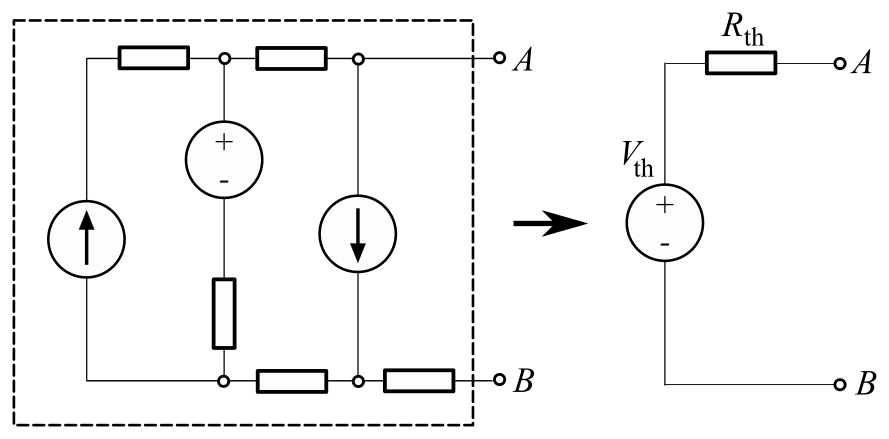
\includegraphics[width=0.5\textwidth]{TheveninEquivalent-1.png}
\caption{Thevenin Equivalent Circuit}
\end{figure}
\end{theorem}
\begin{proof}
This proof is from Paul Horowitz and Winfield Hill, \textit{The Art of Electronics}, 
3rd ed., (Cambridge University Press, New York, 2015), Appendix D.

For linear circuit elements (here resistors), the ``nodal 
equations" (Kirchhoff's voltage law, KVL, and Kirchhoff's current 
law, KCL) are a set of linear equations. So we can
find any circuit quantity (a voltage or a current), which depends 
on all the ``independent sources'' (batteries, current
sources), by turning on each source in turn, and adding the
partial contributions. (This is exactly analogous to using
superposition to find, say, the electric field from a set of
charges.) This technique is often useful in circuit analysis.

Here we wish to mimic the V versus I of the actual circuit 
with the (simpler) Th\'{e}venin equivalent of a single battery 
in series with a single resistor. Imagine we determine
that $V$ versus $I$ function by applying an external current $I_{\rm ext}$
that flows through the two-terminal circuit, and observing
the resultant $V$ across those same two terminals. $V$ depends
on $I_{\rm ext}$ and on all the internal batteries ($V_{\rm int}$) and current
sources ($I_{\rm int}$).
\begin{enumerate}
\item Set all $V_{\rm int}=0$ and all $I_{\rm int}=0$; that is, replace all internal
batteries with short circuits and all current sources with
open circuits. Now, with a given applied I ext , observeV 1 .
\item Define $R_{T} = V_1 /I_{ext} $. (They must be proportional, by linearity.)
\item Now set $I_{ext} = 0$, and turn on the internal batteries and
current sources. Observe $V_2$ , which we will call $V_T$ .
\item Finally, by superposition it must be the case that
\[
V({\rm actual}) =V_1 +V_2 = I_{ext} R_{T} +V_{T} .
\]
\end{enumerate}

This is true for all $I_{ext} $, and is exactly what you get with
the  Th\'{e}venin equivalent circuit, when connected to any
load (which need not be linear).
%; see Figure D.2.
\end{proof}
%To summarize: (a) you determine $R_T$ and $V_T$ by first
%finding the open-circuit voltage, which equals $V_T$ ; then (b)
%you find the short-circuit current, $I_{SC}$ , which equals the
%ratio of $V_T$ to $R_T$ . In other words, $V_T$ = $V _{OC}$ and $R T =
%V OC /I SC$. You do this by analysis, if you know the ``black-
%box" circuit; or by measurement, if you don’t.
%any ``load"
%(not necessarily linear)
%
%Figure D.2. The Thévenin equivalent circuit behaves exactly like
%the original network, regardless of the nature of the load.

For example:
\begin{figure}[H]
\centering
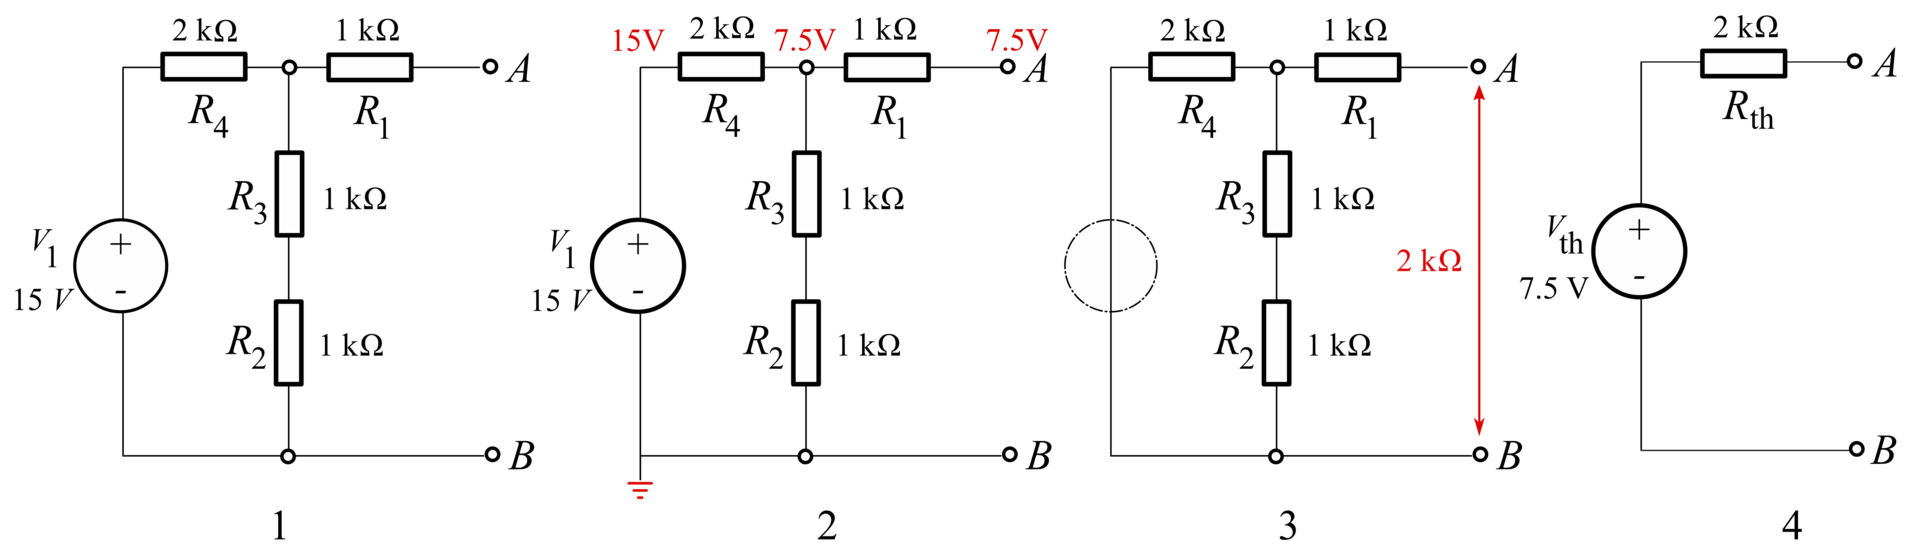
\includegraphics[width=\textwidth]{Thevenin-example-png.png}
\caption{Thevenin's Theorem Example}
\end{figure}

The evaluation process:
\begin{itemize}
\item let A-B be a open circuit and determine the voltages between A-B which is $V_{th}$,
\item then replace all sources as its internal resistance and calculate the resistance between A-B which is $R_{th}$. 
\end{itemize}

\subsubsection{Norton's Theorem}
\begin{theorem}[Norton's Theorem]
~{As the dual of the Thevenin's theorem, Norton's theorem states that any one-port network can be reduced to a single current source and a single impedance. Any black box containing resistances only and voltage and current sources can be replaced by an equivalent circuit consisting of an equivalent current source in parallel connection with an equivalent resistance.}
\begin{itemize}
\item  {Any linear electrical network with voltage and current sources and only resistances can be replaced at terminals A-B by an equivalent current source $I_{no}$ in parallel connection with an equivalent resistance $R_{no}$.}
\item  {This equivalent current $I_{no}$ is the current obtained at terminals A-B of the network with terminals A-B short circuited.}
\item  {This equivalent resistance $R_{no}$ is the resistance obtained at terminals A-B of the network with all its voltage sources short circuited and all its current sources open circuited.}
\end{itemize}
\begin{figure}[H]
\centering
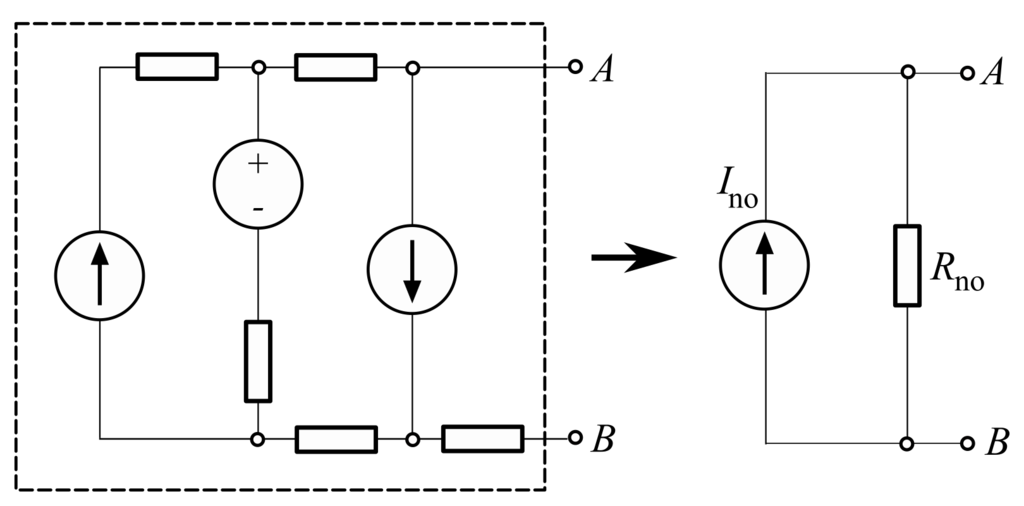
\includegraphics[width=0.5\textwidth]{NortonEquivalentCircuits.png}
\caption{Norton Equivalent Circuit}
\end{figure}
\end{theorem}

For example:
\begin{figure}[H]
\centering
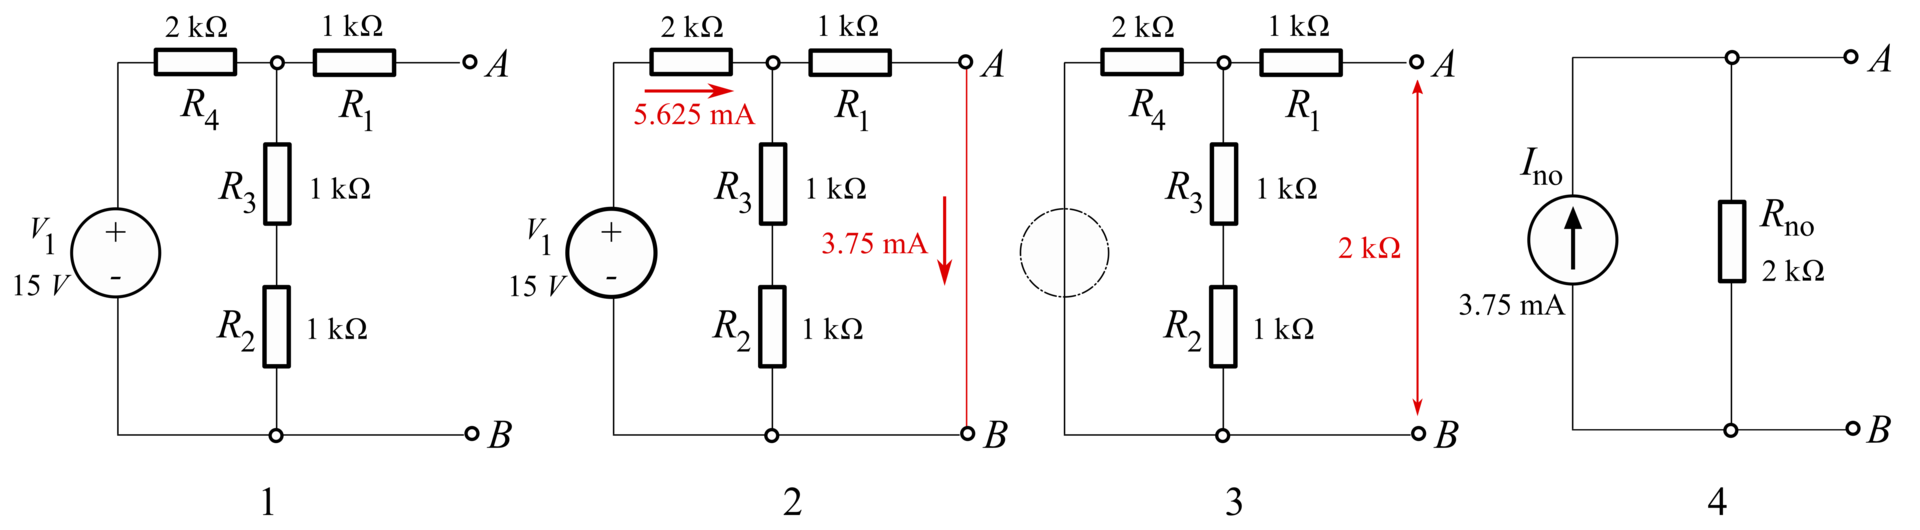
\includegraphics[width=\textwidth]{Norton-example.png}
\caption{Norton's Theorem Example}
\end{figure}

The evaluation process:
\begin{itemize}
\item Find the Norton current $I_{no}$. Calculate the output current, $I_{AB}$, with a short circuit as the load (meaning 0 resistance between A and B). This is $I_{no}$.
\item Find the Norton resistance $R_{no}$. When there are no dependent sources (all current and voltage sources are independent), there are two methods of determining the Norton impedance $R_{no}$.
\begin{enumerate}
\item Calculate the output voltage, $V_{AB}$, when in open circuit condition (i.e., no load resistor – meaning infinite load resistance). $R_{no}$ equals this $V_{AB}$ divided by $I_{no}$.
\item Or replace independent voltage sources with short circuits and independent current sources with open circuits. The total resistance across the output port is the Norton impedance $R_{no}$.
\end{enumerate}
\end{itemize}

\subsubsection{Conversion between both Theorems}
\begin{wrapfigure}{r}{0.5\textwidth}
  \vspace{-50pt}
  \begin{center}
    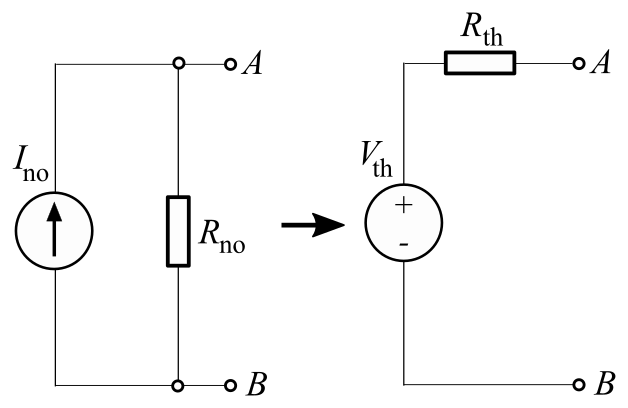
\includegraphics[width=0.48\textwidth]{Norton-to-thevenin.png}
  \end{center}
  \vspace{-20pt}
  \caption{Conversion Demonstration}
  \vspace{-10pt}
\end{wrapfigure}
Both theorem can be converted into each other:
\begin{align*}
R_{th}&=R_{no}\\
V_{th}&=I_{no}R_{no}\\
I_{no}&=\dfrac{V_{th}}{R_{no}}
\end{align*}

\subsection{RLC Circuit Summaries}
%\subsubsection{R Circuit}
%\subsubsection{C Circuit}
%\subsubsection{L Circuit}
\subsubsection{RC Circuit}
 {RC Circuit can be used as the RC filter - high-pass filter:}
\begin{figure}[H]
  \begin{center}    
    \begin{circuitikz}[scale=1]
     	\draw (0,0) to [esource,esource=$V_i$] (0,4);
        \draw (0,4) to [C,C=$C$] (3,4);
        \draw (0,0) to [] (3,0);
        \draw (3,0) to [R,R=$R$] (3,4);
        \draw (3,4) to [] (4,4);
        \draw (3,0) to [] (4,0);
        \draw (4,4) to [open,v=$V_o$] (4,0);
    \end{circuitikz}
    \caption{RC Filter}
  \end{center}
\end{figure}
 {In this RC circuit with $V_i=V_P\sin \omega t$, we can first determine the current and then determine the $V_{out}$}
$$i=\dfrac{V_P}{\sqrt{R^2+\left(\frac{1}{\omega C}\right)^2}}\sin (\omega t+\phi) \qquad \text{where }\phi =\tan ^{-1}\dfrac{1}{\omega CR}$$
\begin{align*}
V_0&=\dfrac{V_PR}{\sqrt{R^2+\left(\frac{1}{\omega C}\right)^2}}\sin (\omega t+\phi)
=\dfrac{V_P\omega CR}{\sqrt{\omega ^2C^2R^2+1}}\sin (\omega t+\phi)\\
&=\dfrac{V_P\omega \tau}{\sqrt{\omega ^2\tau ^2+1}}\sin (\omega t+\phi)
\end{align*}
$$\left|\dfrac{V_o}{V_i}\right|=\sqrt{\dfrac{\omega ^2\tau ^2}{\omega ^2\tau ^2+1}}$$
 {From the expression, we can see that as the increase of frequency, the proportion will increase as well. Therefore, this is a high-pass filter.}
 
 {Also, if we take the output voltage as the capacitor, it becomes the low-pass filter:}
\begin{figure}[H]
  \begin{center}    
    \begin{circuitikz}[scale=1]
     	\draw (0,0) to [esource,esource=$V_i$] (0,4);
        \draw (0,4) to [R,R=$R$] (3,4);
        \draw (0,0) to [] (3,0);
        \draw (3,0) to [C,C=$C$] (3,4);
        \draw (3,4) to [] (4,4);
        \draw (3,0) to [] (4,0);
        \draw (4,4) to [open,v=$V_o$] (4,0);
    \end{circuitikz}
    \caption{RC Filter}
  \end{center}
\end{figure}
$$i=\dfrac{V_P}{\sqrt{R^2+\left(\frac{1}{\omega C}\right)^2}}\sin (\omega t+\phi) \qquad \text{where }\phi =\tan ^{-1}\dfrac{1}{\omega CR}$$
\begin{align*}
V_0 &= \dfrac{1}{C}\int idt 
= \left|V_i\times \dfrac{Z_C}{Z_C+Z_R}\right|
= \dfrac{V_P}{\omega C\sqrt{R^2+\left(\frac{1}{\omega C}\right)^2}}\cos (\omega t+\phi)\\
&= \dfrac{V_P}{\sqrt{\omega ^2C^2R^2+1}}\cos (\omega t+\phi)= \dfrac{V_P}{\sqrt{\omega ^2\tau ^2+1}}\cos (\omega t+\phi)
\end{align*}
\[
\left|\dfrac{V_o}{V_i}\right|=\sqrt{\dfrac{1}{\omega ^2\tau ^2+1}}
\]


\subsubsection{RL Circuit}
RL Circuit can be used as the RL high and low-pass filters:
\begin{figure}[H]
  \begin{center}    
    \begin{circuitikz}[scale=1]
     	\draw (0,0) to [esource,esource=$V_i$] (0,4);
        \draw (0,4) to [L,L=$L$] (3,4);
        \draw (0,0) to [] (3,0);
        \draw (3,0) to [R,R=$R$] (3,4);
        \draw (3,4) to [] (4,4);
        \draw (3,0) to [] (4,0);
        \draw (4,4) to [open,v=$V_o$] (4,0);
    \end{circuitikz}
    \caption{RL low-pass Filter}
  \end{center}
\end{figure}
 {In this RC circuit with $V_i=V_P\sin \omega t$, we can first determine the current and then determine the $V_{out}$}
$$i=\dfrac{V_P}{\sqrt{R^2+\omega ^2L^2}}\sin (\omega t+\phi) \qquad \text{where }\phi =\tan ^{-1}\dfrac{\omega L}{R},$$
\begin{align*}
V_o
&=\dfrac{V_PR}{\sqrt{R^2+\omega ^2L^2}}\sin (\omega t+\phi)
=\dfrac{V_P}{\sqrt{1+\dfrac{\omega ^2L^2}{R^2}}}\sin (\omega t+\phi)
=\dfrac{V_P}{\sqrt{1+\omega ^2\tau ^2}}\sin (\omega t+\phi).
\end{align*}
The voltage magnitude gain is
$$\left|\dfrac{V_o}{V_i}\right|=\sqrt{\dfrac{1}{\omega ^2\tau ^2+1}}.$$
From the expression, we can see that as the decrease of frequency,
the proportion will increase as well. Therefore, this is 
a low-pass filter.
 
Similar to RC circuit, take the output voltage as the inductive, it becomes a high-pass filter.
\begin{figure}[H]
  \begin{center}    
    \begin{circuitikz}[scale=1]
     	\draw (0,0) to [esource,esource=$V_i$] (0,4);
        \draw (0,4) to [R,R=$R$] (3,4);
        \draw (0,0) to [] (3,0);
        \draw (3,0) to [L,L=$L$] (3,4);
        \draw (3,4) to [] (4,4);
        \draw (3,0) to [] (4,0);
        \draw (4,4) to [open,v=$V_o$] (4,0);
    \end{circuitikz}
    \caption{RL high-pass Filter}
  \end{center}
\end{figure}
$$i=\dfrac{V_P}{\sqrt{R^2+\omega ^2L^2}}\sin (\omega t+\phi) \qquad \text{where }\phi =\tan ^{-1}\dfrac{\omega L}{R}$$
\begin{align*}
V_o 
&=\dfrac{1}{L}\dfrac{di}{dt}
=\frac{V_P\omega L}{\sqrt{R^2+\omega ^2L^2}}\cos (\omega t+\phi)
=\frac{V_P \omega \tau}{\sqrt{1+\omega ^2\tau ^2}}\cos (\omega t+\phi)
\end{align*}
$$\left|\dfrac{V_o}{V_i}\right|=\sqrt{\dfrac{\omega ^2\tau ^2}{\omega ^2\tau ^2+1}}$$
\subsubsection{Transfer Function of RC and RL}
\begin{figure}[H]
  \begin{center}    
    \begin{circuitikz}[scale=1]
     	\draw (0,0) to [esource,esource=$V_i$] (0,4);
        \draw (0,4) to [european resistor,european resistor=$Z_1$] (3,4);
        \draw (0,0) to [] (3,0);
        \draw (3,0) to [european resistor,european resistor=$Z_2$] (3,4);
        \draw (3,4) to [] (4,4);
        \draw (3,0) to [] (4,0);
        \draw (4,4) to [open,v=$V_o$] (4,0);
    \end{circuitikz}
    \caption{RC Filter}
  \end{center}
\end{figure}
 {In this circuit, we can use the voltage divider formula to derive the transfer function:}
$$\dfrac{V_o}{V_i}=\dfrac{Z_2}{Z_1+Z_2}$$
\begin{figure}[H]
\centering
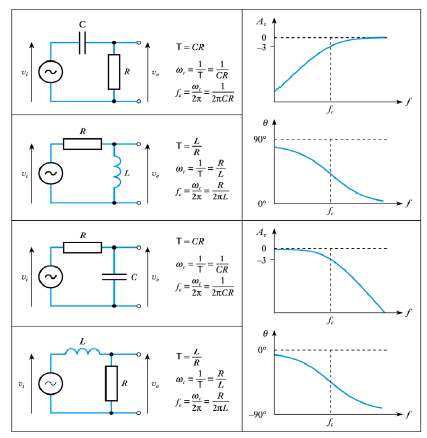
\includegraphics[width=0.8\textwidth]{c2.PNG}
\caption{Comparison of RC-RL Filter}
\end{figure}
\subsubsection{RLC Circuit}
\begin{itemize}
\item RLC in Series
\begin{figure}[htbp]
  \begin{center}    
    \begin{circuitikz}[scale=1]
     	\draw (0,0) to [esource,esource=$V_i$] (0,4);
        \draw (0,4) to [european resistor,european resistor=$R$] (3,4);
        \draw (0,0) to [L,L=$L$] (3,0);
        \draw (3,0) to [C,C=$C$] (3,4);
        \draw (3,4) to [] (4,4);
        \draw (3,0) to [] (4,0);
        \draw (4,4) to [open,v=$V_C$] (4,0);
    \end{circuitikz}
    \caption{RLC Resonant Circuit}
  \end{center}
\end{figure}
$$Z=Z_R+Z_C+Z_L=R+j\omega L-j\dfrac{1}{\omega C}$$
 {When the reactance becomes zero:}
$$\omega L=\dfrac{1}{\omega C} \implies \omega _0=\dfrac{1}{\sqrt{LC}}$$
 {Assuming the $V_C=A\sin \omega t$, the current $i$ can be determined:}
$$i=C\dfrac{dV}{dt}=C\dfrac{d}{dt}A\sin \omega t=A\omega C\cos \omega t$$
 {therefore, as the definition of the quality factor which can be determined as the following:}
\begin{align*}
Q&=2\pi \dfrac{\text{Max of the energy store}}{\text{dissipated energy in resonant circle}}\\
&=2\pi \dfrac{E_S}{E_D}=2\pi \dfrac{\frac{1}{2}Li^2+\frac{1}{2}CV^2}{R \langle i^2 \rangle }
=2\pi \dfrac{\dfrac{1}{2}L\omega ^2C^2A^2\cos ^2\omega t+\dfrac{1}{2}CA^2\sin ^2\omega t}{R\dfrac{\omega _0^2C^2A^2}{2}\dfrac{2\pi}{\omega _0}}\\
&=2\pi \dfrac{\dfrac{1}{2}CA^2}{R\dfrac{\omega _0^2C^2A^2}{2}\dfrac{2\pi}{\omega _0}}=\dfrac{1}{\omega _0RC}
\end{align*}
\item RLC in Parallel
\begin{figure}[htbp]
  \begin{center}    
    \begin{circuitikz}[scale=1]
     	\draw (0,0) to [sV,sV=$V_i$] (0,4);
        \draw (2,4) to [C,C=$C$] (2,0);
        \draw (4,4) to [L,L=$L$] (4,0);
        \draw (6,4) to [european resistor,european resistor=$R$] (6,0);
        \draw (0,0) to [] (6,0);
        \draw (0,4) to [] (6,4);
    \end{circuitikz}
    \caption{RLC Resonant Circuit}
  \end{center}
\end{figure}
$$\dfrac{1}{Z}=\dfrac{1}{Z_C}+\dfrac{1}{Z_L}+\dfrac{1}{Z_R}$$
$$Z=\dfrac{R}{1+jR(\omega C-1/\omega L)}$$
$$\omega _0=\dfrac{1}{\sqrt{LC}}$$
 {Assuming that the voltage across the capacitor is $V_C=A\sin \omega t$, then the current across the inductive is $i=\dfrac{1}{L}\int V_cdt=\dfrac{-A}{\omega L}\cos \omega t$ and then we can determine the quality factor:}
\begin{align*}
Q&=2\pi \dfrac{E_S}{E_D}=2\pi \dfrac{\frac{1}{2}Li^2+\frac{1}{2}CV^2}{\dfrac{<V^2>}{R}}\\
&=2\pi \dfrac{\frac{1}{2}L(\dfrac{-A}{\omega L}\cos \omega t)^2+\frac{1}{2}C(A\sin \omega t)^2}{\dfrac{A^2}{2R}\dfrac{2\pi}{\omega _0}}\\
&=2\pi \dfrac{\frac{1}{2}CA^2}{\dfrac{A^2}{2R}\dfrac{2\pi}{\omega _0}}=\omega _0 RC
\end{align*}
 {And for the bandwidth, it can be shown that: }
$$Q=\dfrac{\omega _0}{\Delta\omega }$$
\end{itemize}

\subsection{Transient Response in RL, RC and RLC Circuit}
\subsubsection{Charging and Discharging Capacitor}
\begin{itemize}
\item Charging Capacitor
\begin{figure}[H]
\centering
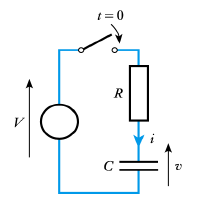
\includegraphics[scale=0.9]{a1.PNG}
\caption{Charging Capacitor}
\end{figure}
$$V=V(1-e^{-\dfrac{t}{RC}})=V(1-e^{-\dfrac{t}{\tau}}) \qquad \tau =\dfrac{1}{RC}$$
$$i=ie^{-\dfrac{t}{RC}}=\dfrac{V}{R}e^{-\dfrac{t}{\tau}}$$
\begin{figure}[H]
\centering
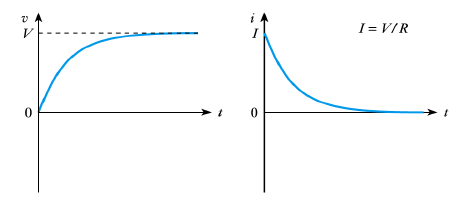
\includegraphics[scale=0.9]{a2.PNG}
\caption{Charging Capacitor}
\end{figure}
\item Discharging Capacitor
\begin{figure}[H]
\centering
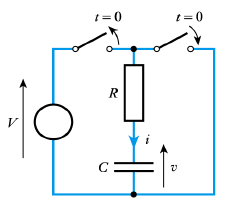
\includegraphics[scale=0.9]{a3.PNG}
\caption{Discharging Capacitor}
\end{figure}
$$V=Ve^{-\dfrac{t}{RC}}=Ve^{-\dfrac{t}{\tau}}$$
$$i=-ie^{-\dfrac{t}{RC}}=-\dfrac{V}{R}e^{-\dfrac{t}{\tau}}$$
\begin{figure}[H]
\centering
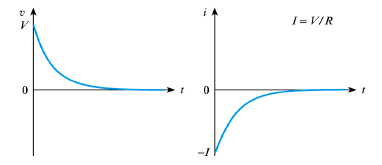
\includegraphics[scale=0.9]{a4.PNG}
\caption{Discharging Capacitor}
\end{figure}
\end{itemize}
\subsubsection{Energizing and De-energizing Inductor}
\begin{itemize}
\item Energizing Inductor
\begin{figure}[H]
\centering
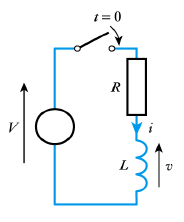
\includegraphics[scale=0.9]{b1.PNG}
\caption{Energizing Inductor}
\end{figure}
$$V=Ve^{-\dfrac{Rt}{L}}=Ve^{-\dfrac{t}{\tau}} \qquad \tau =\dfrac{L}{R}$$
$$i=\dfrac{V}{R}(1-e^{-\dfrac{Rt}{L}})=\dfrac{V}{R}(1-e^{-\dfrac{t}{\tau}})$$
\begin{figure}[H]
\centering
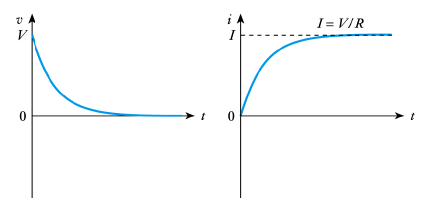
\includegraphics[scale=0.9]{b2.PNG}
\caption{Energizing Inductor}
\end{figure}
\item De-energizing Inductor
\begin{figure}[H]
\centering
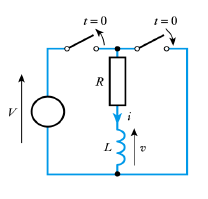
\includegraphics[scale=0.9]{b3.PNG}
\caption{De-energizing Inductor}
\end{figure}
$$V=-Ve^{-\dfrac{Rt}{L}}=-Ve^{-\dfrac{t}{\tau}}$$
$$i=\dfrac{V}{R}e^{-\dfrac{Rt}{L}}=\dfrac{V}{R}e^{-\dfrac{t}{\tau}}$$
\begin{figure}[H]
\centering
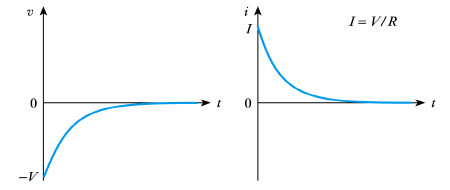
\includegraphics[scale=0.9]{b4.PNG}
\caption{De-energizing Inductor}
\end{figure}
\end{itemize}

\subsubsection{Response for the First Order System}
Initial and final value formulae:
$$V=V_f+(V_i-V_f)e^{-\dfrac{t}{\tau}}$$
$$i=i_f+(i_i-i_f)e^{-\dfrac{t}{\tau}}$$
 {The first term in each case is the \textbf{steady-state response}}\\
 {The second term represents the \textbf{transient response}}\\
 {The combination gives the \textbf{total response} of the arrangement}

\subsubsection{Response for the Second Order System}
$$\dfrac{1}{\omega _n^2}\dfrac{d^2y}{dt^2}+\dfrac{2\zeta }{\omega _n}\dfrac{dy}{dt}+y=x$$
 {For this second order differential equation, we have:}
\begin{align*}
\omega _n & \text{ is the \textbf{undamped natural frequency} (rad/s)}\\
\zeta & \text{ is the \textbf{damping factor}}
\end{align*}

\subsubsection{Graph}
\begin{figure}[H]
\centering
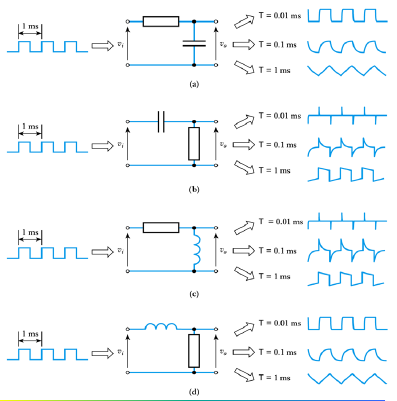
\includegraphics[scale=1.2]{c3.PNG}
\caption{Output of first-order systems to a square waves - for different time response}
\end{figure}
\begin{figure}[H]
\centering
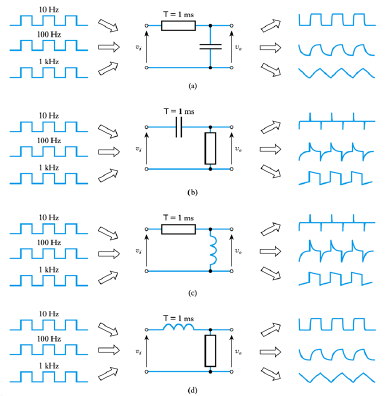
\includegraphics[scale=1.2]{c4.PNG}
\caption{Output of first-order systems to a square waves - for different frequencies}
\end{figure}
\end{document}
